\documentclass[11pt]{article}

% Page format
\usepackage[margin=1in]{geometry}

% Math packages and custom commands 
\usepackage{framed, tikz}
\usepackage[utf8]{inputenc}
\usepackage{mathtools,amsthm}
\usepackage{enumitem,amssymb}
\usepackage{hyperref}
\usepackage{graphicx}

\definecolor{shadecolor}{gray}{0.9}


\newtheoremstyle{case}{}{}{}{}{}{:}{}{}
\theoremstyle{case}
\newtheorem{case}{Case}
\DeclareMathOperator{\R}{\mathbb{R}}
\DeclareMathOperator{\E}{\mathbb{E}}
\DeclareMathOperator{\Var}{\text{Var}}
\DeclareMathOperator{\Cov}{\text{Cov}}
\newcommand{\bvec}[1]{\mathbf{#1}}
\renewcommand{\P}{\mathbb{P}}
\newcommand{\norm}[2][2]{\| #2\|}
\newcommand{\note}[1]{\noindent{[\textbf{NOTE:} #1]}}
\newcommand{\hint}[1]{\noindent{[\textbf{HINT:} #1]}}
\newcommand{\recall}[1]{\noindent{[\textbf{RECALL:} #1]}}

\DeclareMathOperator*{\argmin}{arg\,min}
\DeclareMathOperator*{\argmax}{arg\,max}


\begin{document}

\begin{center}
{\Large CSCE 790-003, Spring 2022 \\ Assignment 2}

\begin{tabular}{rl}
Username: & [your email username] \\
Name: & [your first and last name] \\
\end{tabular}
\end{center}
By turning in this assignment, I agree by the honor code of USC Columbia.

\paragraph{Submission.}
You need to submit the following files to Blackboard:
\begin{itemize}
    \item A pdf file named as assignment2\_$\langle username \rangle$.pdf, where you replace $\langle username \rangle$ with your email username. This pdf file contains your answers to the written problems, including problems 1, 3, and written problems of problem 2. Edit the assignment2.tex file (or scan your handwritten script) to fill in your answers, and submit the pdf file generated from the edited tex file.
    \item A zip file named as assignment2\_$\langle username \rangle$.zip, where you replace $\langle username \rangle$ with your email username. This zip file contains the three .py files you will edit for problem 2.
\end{itemize}

\section{$\epsilon$-greedy Policy Improvement [25pt]}
Prove the $\epsilon$-greedy policy improvement theorem mentioned in class:
Fix some $\epsilon\in[0,1]$.
Let $\pi$ be the $\epsilon$-greedy policy wrt some arbitrary $Q\in\mathbb{R}^{|S||A|}$, and let $\pi'$ be the $\epsilon$-greedy policy wrt $Q^\pi$.
Then, $V^{\pi'}(s) \geq V^{\pi}(s) ~\forall s$.

\underline{Hint:}
Due to the policy difference lemma (Problem 2a of Assignment 1), it is sufficient to show that $A^\pi(s,\pi') = \sum_{a} \pi'(a|s)Q^\pi(s,a) - \sum_{a} \pi(a|s)Q^\pi(s,a) \geq 0 ~\forall s$.
Also, you might need to use this inequality:
\begin{align*}
   \max_a Q^\pi(s,a) \geq \sum_a \frac{\pi(a|s)-\frac{\epsilon}{|A|}}{1-\epsilon} Q^\pi(s,a).
\end{align*}
If you use it, explain why it holds first.

\begin{shaded}

\begin{align*}
\pi'(a|s) = 
	\begin{cases}
	& \frac{\epsilon}{|A|} + 1 -\epsilon, \text {if }a = \arg \max_a Q^\pi(s,a)\\
	& \frac{\epsilon}{|A|}, \text {otherwise} \\
	\end{cases}
\end{align*}

\begin{align*}
   Q^{\pi}(s,\pi'(s)) & = \sum_{a \in A} \pi'(a|s) Q^{\pi}(s,a) \\
					& = \sum_{a \in A, a \neq \arg \max_a Q^\pi(s,a)}  \frac{\epsilon}{|A|} Q^{\pi}(s,a) + (\frac{\epsilon}{|A|}+1- \epsilon) \max_a  Q^\pi(s,a)\\
					& = \frac{\epsilon}{|A|} \sum_{a \in A}  Q^{\pi}(s,a) + (1- \epsilon) \max_a Q^\pi(s,a) \\	
					& \geq \frac{\epsilon}{|A|} \sum_{a \in A} Q^{\pi}(s,a) + (1- \epsilon)  \sum_a \frac{\pi(a|s)-\frac{\epsilon}{|A|}}{1-\epsilon} Q^\pi(s,a) \\
					& =  \sum_{a \in A} \pi(a|s) Q^{\pi}(s,a)  = V^{\pi}(s)
\end{align*}

As we have $\pi$ be the $\epsilon$-greedy policy wrt some arbitrary $Q\in\mathbb{R}^{|S||A|}$:
\begin{align*}
   &\sum_a \frac{\pi(a|s)-\frac{\epsilon}{|A|}}{1-\epsilon} Q^\pi(s,a)\\
= &  \frac{ \sum_{a \in A, a \neq \arg \max_a Q^\pi(s,a) } (\pi(a|s)-\frac{\epsilon}{|A|}) Q^\pi(s,a) + (\pi(a|s)-\frac{\epsilon}{|A|}) \max_a Q^\pi(s,a)}{1-\epsilon} \\
\leq &  \frac{ \sum_{a \in A, a \neq \arg \max_a Q^\pi(s,a) } (\frac{\epsilon}{|A|}-\frac{\epsilon}{|A|}) Q^\pi(s,a) + (\frac{\epsilon}{|A|} + 1 -\epsilon-\frac{\epsilon}{|A|}) \max_a Q^\pi(s,a)}{1-\epsilon} \\
= &  \frac{ (\frac{\epsilon}{|A|} + 1 -\epsilon-\frac{\epsilon}{|A|}) \max_a Q^\pi(s,a)}{1-\epsilon} \\
=  & \max_a Q^\pi(s,a)
\end{align*}
The equality is satisfied when the max action under $\pi'$ is the same as $\pi$, namely $a_0: \max_{a\in A} ^\pi(s,a)=q^\pi(s,a_0)$. The inequality is satisfied when the max action under $\pi'$ is not $a_0$ in which case: $\max_{a\in A} ^\pi(s,a) > q^\pi(s,a_0)$.

\end{shaded}

\newpage
\section{Implementing Q-learning [75pt]}


This problem is adapted from Emma Brunskill's course.

In this problem, we will implement variants of Q-learning, including tabular Q-learning, Q-learning with linear function approximators, and Deep Q-Network (DQN).
Your implementation will be tested on a test environment on your local computer with CPU and OpenAI gym's \texttt{Pong-v0} environment (an Atari game) on the recommended platform, Google Colab.

The starter code is in folder \texttt{starter\_code\_torch}.

\paragraph{Working locally.}
Please be sure you have Anaconda or Miniconda installed.
Create conda environment on your local system: replace \texttt{<your-system>} with your system, either mac or windows:

    \texttt{cd starter\_code\_torch}
    
    \texttt{conda env create -f cs234-torch-<your-system>.yml}
    
    \texttt{conda activate cs234-torch}


\paragraph{Working remotely on Google Colab.}
If you are not familiar with Google Colab, just create an account at Google Colab and follow the tutorials. Google Colab is very nice to run Python code without the hassle of installing libraries and to leverage a GPU or TPU.

\subsection{Test environment [10pt]}
\label{sec:Test environment}
Before running our code on Pong, it is crucial to test our code on a test environment. In this problem, you will reason about optimality in the provided test environment by hand; later, to sanity-check your code, you will verify that your implementation is able to achieve this optimality. You should be able to run your models on CPU in no more than a few minutes on the following environment:

\begin{itemize}
	\item $ 4 $ states: $ 0, 1, 2, 3 $
	\item $ 5 $ actions: $ 0, 1, 2, 3, 4 $. Action $ 0 \leq i \leq 3 $ goes to state $ i $, while action $ 4 $ makes the agent stay in the same state.
	\item Rewards: Going to state $ i $ from states 0, 1, and 3 gives a reward $R(i) $, where $R(0) = 0.2, R(1) = -0.1, R(2) = 0.0, R(3) = -0.3 $. If we start in state $ 2 $, then the rewards defined above are multiplied by $ - 10 $.  See Table~\ref{tab:TestEnv} for the full transition and reward structure. 
	\item One episode lasts 5 time steps (for a total of 5 actions) and always starts in state $ 0 $ (no rewards at the initial state).        
\end{itemize}

\begin{table}[h]
    \centering
    \begin{tabular}{ | l | l | l | l |}  
		\hline
		State ($s$) & Action ($a$) & Next State ($s'$) & Reward ($R$) \\ \hline
		0 & 0 & 0 & 0.2    \\ \hline
		0 & 1 & 1 & -0.1   \\ \hline
		0 & 2 & 2 & 0.0 \\ \hline
		0 & 3 & 3 & -0.3 \\ \hline
		0 & 4 & 0 & 0.2 \\ \hline
		1 & 0 & 0 & 0.2    \\ \hline
		1 & 1 & 1 & -0.1   \\ \hline
		1 & 2 & 2 & 0.0 \\ \hline
		1 & 3 & 3 & -0.3 \\ \hline
		1 & 4 & 1 & -0.1 \\ \hline
		2 & 0 & 0 & -2.0    \\ \hline
		2 & 1 & 1 & 1.0   \\ \hline
		2 & 2 & 2 & 0.0 \\ \hline
		2 & 3 & 3 & 3.0 \\ \hline
		2 & 4 & 2 & 0.0 \\ \hline
		3 & 0 & 0 & 0.2    \\ \hline
		3 & 1 & 1 & -0.1   \\ \hline
		3 & 2 & 2 & 0.0 \\ \hline
		3 & 3 & 3 & -0.3 \\ \hline
		3 & 4 & 3 & -0.3 \\ \hline    
	\end{tabular}
    \caption{Transition table for the Test Environment}
    \label{tab:TestEnv} 
\end{table}


An example of a trajectory (or episode) in the test environment is shown in Figure \ref{fig:test_env}, and the trajectory can be represented in terms of $s_t, a_t, R_t$ as: 
$s_0 = 0, a_0=1, R_0 = -0.1, s_1=1, a_1=2, R_1 = 0.0, s_2=2, a_2=4, R_2 = 0.0, s_3=2, a_3=3, R_3  = 3.0, s_4=3, a_4=0, R_4 = 0.2, s_5=0 $.

\begin{figure}[h!]
  \centering
  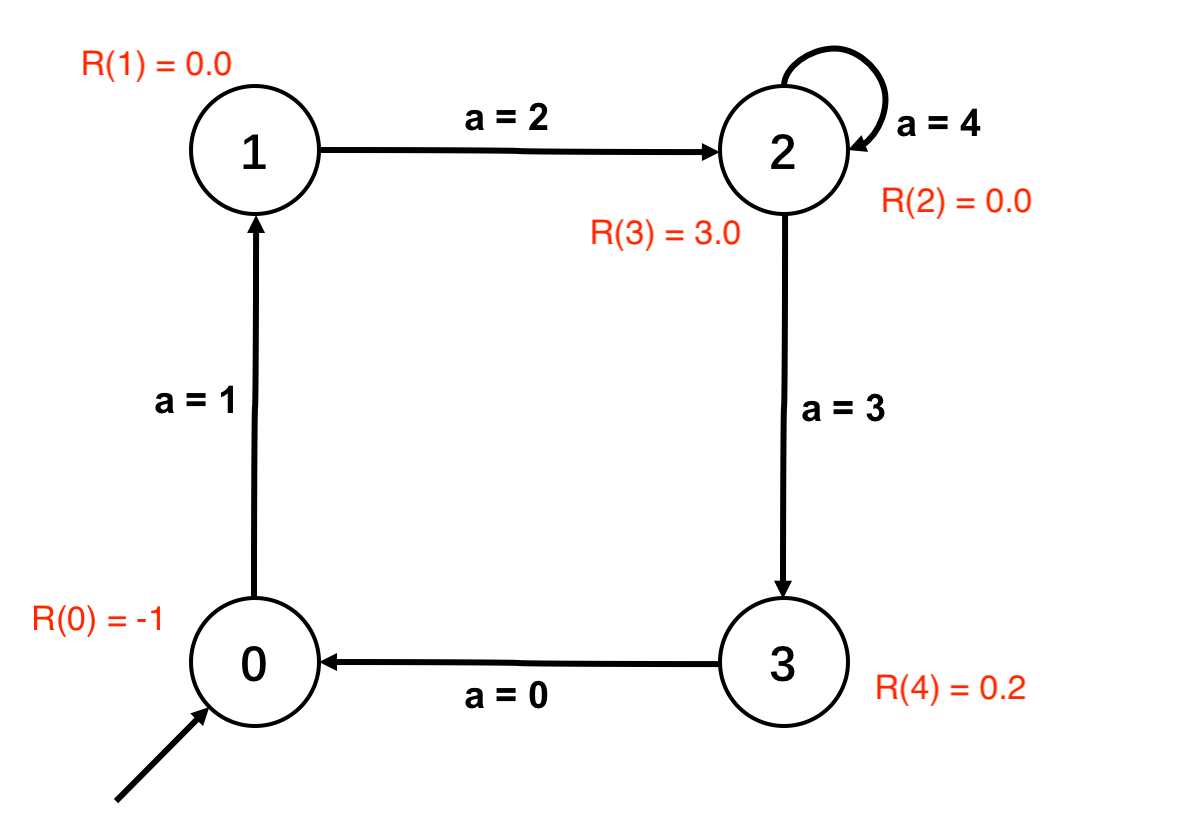
\includegraphics[width=.45\linewidth]{test_env.png}
  \caption{Example of a trajectory in the Test Environment}
  \label{fig:test_env}
\end{figure}

({\bf writing}) What is the maximum sum of rewards that can be achieved in a single trajectory in the test environment, assuming $\gamma = 1$? Show first that this value is attainable in a single trajectory, and then briefly argue why no other trajectory can achieve greater cumulative reward.
\begin{shaded}
We start by $s_0$ , take action 2, then goes to $s_2$, then take action 3, goes to $s_3$, then take action 2, goes to $s_2$, then take action 3, goes to $s_3$, then take action 0, goes to $s_0$.\\
We get a sum of 6.2 reward. If we do not go through state 2, then the maximum reward we can get in one action is 0.2, getting it 5 time steps in a row still can't compare with the 3 reward from state 2 to state 3.
\end{shaded}

\subsection{Tabular Q-learning [15pt]}
If the state and action spaces are sufficiently small, we can simply maintain a table containing the value of $Q(s,a)$, an estimate of $Q^*(s,a)$, for every $(s,a)$ pair.
In this \emph{tabular setting}, given an experience sample $(s, a, r, s')$, the update rule is
\begin{equation}
Q(s,a) \leftarrow Q(s,a) + \alpha\left(r + \gamma \max_{a' \in \mathcal{A}}Q(s',a') - Q(s,a)\right) \label{eqn:tabularq}
\end{equation}
where $\alpha > 0$ is the learning rate, $\gamma \in [0,1)$ the discount factor.

For exploration, we use an $\epsilon$-greedy strategy.
This means that with probability $\epsilon$, an action is chosen uniformly at random from $\mathcal{A}$, and with probability $1-\epsilon$, the greedy action (i.e., $\arg\max_{a \in \mathcal{A}} Q(s,a)$) is chosen.

({\bf coding}) Implement the \texttt{get\_action} and \texttt{update} functions in \texttt{q2\_schedule.py}. Test your implementation by running \texttt{python q2\_schedule.py}.
Include your \texttt{q2\_schedule.py} in the zip file for submission.


\subsection{Q-Learning with Function Approximation [30pt]} 
Due to the scale of Atari environments, we cannot reasonably learn and store a Q value for each state-action tuple. We will instead represent our Q values as a parametric function $Q_{\theta}(s,a)$ where $\theta \in \mathbb{R}^p$ are the parameters of the function (typically the weights and biases of a linear function or a neural network). In this \emph{approximation setting}, the update rule becomes
\begin{equation}
\theta \leftarrow \theta + \alpha\left(r+\gamma \max_{a' \in \mathcal{A}} Q_{\theta}(s', a') - Q_{\theta}(s, a)\right) \nabla_{\theta}Q_{\theta}(s, a) \label{eqn:faq}
\end{equation}
where $(s,a,r,s')$ is a transition from the MDP.\\

To improve the data efficiency and stability of the training process, DeepMind's DQN employed two strategies:
\begin{itemize}
	\item A \textit{replay buffer} to store transitions observed during training. When updating the $Q$ function, transitions are drawn from this replay buffer. This improves data efficiency by allowing each transition to be used in multiple updates.
	
	\item A \textit{target network} with parameters $\bar{\theta}$ to compute the target value of the next state, $\max_{a'} Q(s',a')$. The update becomes
	\begin{equation}
	\theta \leftarrow \theta + \alpha\left(r+\gamma \max_{a' \in \mathcal{A}}Q_{\bar{\theta}}\left(s', a'\right) - Q_{\theta}(s, a)\right) \nabla_{\theta} Q_{\theta}(s, a) \label{eqn:target-update}
	\end{equation}
\end{itemize}

Updates of the form \eqref{eqn:target-update} applied to transitions sampled from a replay buffer $\mathcal{D}$ can be interpreted as performing stochastic gradient descent on the following objective function: 
\begin{equation}
L_{\text{DQN}}(\theta) = \underset{(s,a,r,s') \sim \mathcal{D}}{\mathbb{E}}\left[\left(r+\gamma \max_{a' \in \mathcal{A}}Q_{\bar{\theta}}(s', a') - Q_{\theta}(s, a)\right)^2\right] \label{eqn:brm}
\end{equation}
Note that this objective is also a function of both the replay buffer $\mathcal{D}$ and the target network $Q_{\bar{\theta}}$.
The target network parameters $\bar{\theta}$ are held fixed and not updated by SGD, but periodically -- every $C$ steps -- we synchronize by copying $\bar{\theta} \leftarrow \theta$.

\begin{enumerate}[label=(\alph*)]
    \item ({\bf coding}) We will now implement linear approximation in PyTorch. This question will set up the pipeline for the remainder of the assignment. You'll need to implement the following functions in \texttt{q3\_linear\_torch.py} (please read through \texttt{q3\_linear\_torch.py}):
    \begin{itemize}
    	\item \texttt{initialize\_models}
    	\item \texttt{get\_q\_values}
    	\item \texttt{update\_target}
    	\item \texttt{calc\_loss}
    	\item \texttt{add\_optimizer}
    \end{itemize}
    Test your code by running \texttt{python q3\_linear\_torch.py} \textbf{locally on CPU}.  This will run linear approximation with PyTorch on the test environment from \ref{sec:Test environment}.  Running this implementation should only take a minute.
    Include your \texttt{q3\_linear\_torch.py} in the zip file for submission.
    
    \item ({\bf writing}) Do you reach the optimal achievable reward on the test environment? Attach the plot \texttt{scores.png} from the directory \texttt{results/q3\_linear} to your writeup.
    \begin{shaded}
	The score against epochs:\\
    \begin{minipage}{1\linewidth}\centering
	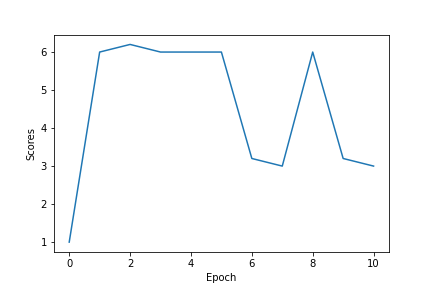
\includegraphics[width=0.80\linewidth]{./starter_code_torch/results/q3_linear/scores.png}
	\end{minipage}
	It sometimes reached the optimal 6.2, but was not stable.
    \end{shaded}
    
    \item ({\bf coding}) Implement the deep Q-network as described in by implementing \texttt{initialize\_models} and \texttt{get\_q\_values} in \texttt{q4\_nature\_torch.py}. The rest of the code inherits from what you wrote for linear approximation. Test your implementation \textbf{locally on CPU} on the test environment by running \texttt{python q4\_nature\_torch.py}.  Running this implementation should only take a minute or two.
    Include your \texttt{python q4\_nature\_torch.py} in the zip file for submission.
    
    \item ({\bf writing}) Attach the plot of scores, \texttt{scores.png}, from the directory \texttt{results/q4\_nature} to your writeup. Compare this model with linear approximation. How do the final performances compare? How about the training time?
    \begin{shaded}
    \begin{minipage}{1\linewidth}\centering
	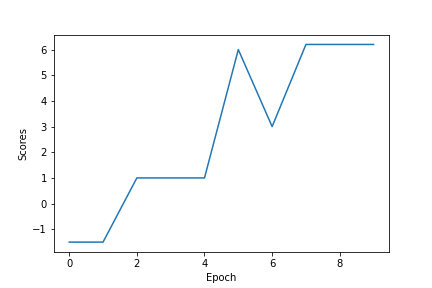
\includegraphics[width=0.80\linewidth]{./starter_code_torch/results/q4_nature/scores.png}
	\end{minipage}
    \end{shaded}
	The DQN is faster to my suprise, and it stay at the optimal.
\end{enumerate}

\newpage

\subsection{DQN on Atari [20pt]} 
The \texttt{Pong-v0} environment from OpenAI gym returns observations (or original frames) of size $ (210 \times 160 \times 3) $, the last dimension corresponds to the RGB channels filled with values between $ 0 $ and $ 255 $ (\texttt{uint8}). Following the DQN paper, we will apply some preprocessing to the observations:

\begin{itemize}
    \item Single frame encoding: To encode a single frame, we take the maximum value for each pixel color value over the frame being encoded and the previous frame. In other words, we return a pixel-wise max-pooling of the last 2 observations.  
    \item Dimensionality reduction: Convert the encoded frame to grey scale, and rescale it to $(80 \times 80 \times 1)$. (See Figure \ref{fig:pong_grey})
\end{itemize}

The above preprocessing is applied to the 4 most recent observations and these encoded frames are stacked together to produce the input (of shape $(80 \times 80 \times 4)$) to the Q-function. Also, for each time we decide on an action, we perform that action for 4 time steps. This reduces the frequency of decisions without impacting the performance too much and enables us to play 4 times as many games while training.

\begin{figure}[h!]
  \centering
  
\includegraphics[width=.3\linewidth]{pong.jpg}
  \caption{Original input $ (210 \times 160 \times 3) $ with RGB colors}
  \label{fig:pong}
\end{figure}

\begin{figure}[h!]
  \centering
  
\includegraphics[width=.3\linewidth]{pong_grey.png}
  \caption{After preprocessing in grey scale of shape $ (80 \times 80 \times 1 ) $}
  \label{fig:pong_grey}
\end{figure}

\begin{enumerate}[label=(\alph*)]
\item (\textbf{coding and written}). Now we're ready to train on the Atari \texttt{Pong-v0} environment. First, launch linear approximation on pong with \texttt{python q5\_train\_atari\_linear.py} \textbf{(recommended on Google Colab's GPU)}. This will train the model for 500,000 steps and should take approximately an hour.  Briefly qualitatively describe how your agent's performance changes over the course of training. Do you think that training for a larger number of steps would likely yield further improvements in performance? Explain your answer.
\begin{shaded}
I tried several ways, but the terminal did not start training, the code I wrote, however, is correct. 
\end{shaded}

\item (\textbf{coding and written}). In this question, we'll train the agent with DeepMind's architecture on the Atari \texttt{Pong-v0} environment. Run \texttt{python q6\_train\_atari\_nature.py} \textbf{(recommended on Google Colab's GPU)}.  This will train the model for 4 million steps. To speed up training, we have trained the model for 2 million steps. You are responsible for training it to completion, which should take \textbf{12 hours}. Attach the plot \texttt{scores.png} from the directory \texttt{results/q6\_train\_atari\_nature} to your writeup.
You should get a score of around 11-13 after 4 million total time steps.  As stated previously, the DeepMind paper claims average human performance is $ -3 $.
\begin{shaded}
Your answer here.
\end{shaded}

\end{enumerate}



\end{document}